\section{Evaluation}
\label{sec:eval}
In this section, we introduce the dataset and experimental setup. We analyze the results and show the advantages of our approach~\footnote{Data and source code are available at: \url{https://anonymous.4open.science/r/SemiSum}}.

\subsection{Datasets}
In this experiment, we use the following three datasets.

\textbf{Yelp} 
\footnote{\url{https://www.yelp.com/dataset}}
contains a large number of reviews about consumer services on Yelp. 
\citet{MeanSum19} released the development and test set in which each sample 
has 8 reviews about a business outlet and one human-written summary about them.

\textbf{Amazon} 
\footnote{\url{https://cseweb.ucsd.edu/~jmcauley/datasets.html}}
is a dataset~\cite{HeM16} made up of product reviews from four different product categories. 
Each sample in development and test set consists of 8 reviews and 3 human-written summaries~\cite{Copycat20}. 

\textbf{RottenTomatoes} (RT) ~\cite{RT16}
~\footnote{\url{https://web.eecs.umich.edu/~wangluxy/data.html}}
is a large set of movie reviews. Each set of reviews about a
movie has a gold summary written by an editor. However, we do not use the gold summaries for training, 
because we are targetting an unsupervised setting.

For training, we construct the synthetic semi-structured training set for these three datasets.
Human-annotated multi-review and summary pairs
are used as development set and testing set.  
Details are shown in \tabref{tab:datasets}
\footnote{The size of our synthetic training set does not exceed that of the synthetic training set created by previous methods in \tabref{sec:base}.}.

\begin{table}[th]
	\small
	\centering
	\begin{tabular}{|l|c|c|c|}
		\hline
		\textbf{} & \textbf{Training} &\textbf{Development} & \textbf{Testing}\\
		\hline
		Yelp & 100k & 100 & 100 \\
		Amazon & 90k & $28\times3$ & $32\times3$ \\
		RT & 25k& 536 & 737\\
		\hline
	\end{tabular}
	\caption{%Data statistics show 
		The number of  train/dev/test pairs. 
		The training column shows the number of our synthetic semi-structured training pairs.
		%\KZ{But when you compare with other baselines, how much training data do they use?} 
		$\times3$ means 3 human-written summaries per multi-review.}
	\label{tab:datasets}
\end{table}

\subsection{Models under Comparison}
\label{sec:base}
We compared different methods trained on their own synthetic training data.
The brief descriptions are listed as follows:
%\cut{%%
\begin{itemize}
	\item \textbf{MeanSum}~\cite{MeanSum19} was an unsupervised auto-encoder model, which decodes the summary based on the mean representation of input reviews.
	\item \textbf{CopyCat}~\cite{Copycat20} used a hierarchical variational autoencoder model with the controlling of novelty between inputs and the generated review.
	\item \textbf{OpiDig}~\cite{OpiDig20} took a review as output and the OAs of this review as input for training. At test, it selected the important OAs from the multi-reviews
	and generated summaries.
	\item \textbf{Denoise}~\cite{Denoise20} presented a denoising summarization model with linguistically motivated noising datasets.
	\item \textbf{FewSum}~\cite{Fewshot20} was a conditional transformer model specially designed on consideration of review properties, including content coverage, writing style and length deviations.
	\item \textbf{PlanSum}~\cite{Plansum20} trained sentiment and aspect distributions for synthetic dataset construction and summary generation.
	\item \textbf{TranSum}~\cite{transsum21} trained sentiment and aspect embeddings as review embeddings and used these embeddings as input of the summarization model.
	%and computed the distance between summary and all remaining reviews as weights of review embeddings for summarization.
\end{itemize}
%}%%%
Both PlanSum and TranSum 
%obtained sentiment and aspect representation of reviews by different training methods,
%which both 
need human to annotate sentiment labels
for each review in the corpus.
However, our approach only needs reviews without any other human-annotated labels.

In the following experiments, we denote the basic aspect-guided model as {\bf BM}, 
the advanced aspect-guided model as {\bf AM}, 
and the training of advanced model initialized with pretrained basic model as {\bf TBA}. TBA has two variants: TBA-T which 
stands for TBA based on non-pretrained Transformer~\cite{Transformer17}, and TBA-B which stands for TBA based on pretrained BART~\cite{BART20}
\footnote{https://github.com/pytorch/fairseq}.

\begin{table*}[t]
	\centering
	%\small
	\begin{tabular}{|l|ccccc|ccccc|ccccc|}
		\hline
		\multirow{2}{*}{\bf Approach} & \multicolumn{5}{c|}{\bf Yelp} &  \multicolumn{5}{c|}{\bf Amazon} & \multicolumn{5}{c|}{\bf RT} \\ \cline{2-16}
		& R-1 & R-2 & R-L& AC &Div$\downarrow$ & R-1 & R-2 & R-L& AC & Div$\downarrow$ & R-1 & R-2 & R-L& AC & Div$\downarrow$\\
		\hline
		Meansum & 28.86 & 3.66 & 15.19 & 0.34 & 0.38 &  29.20 &4.70 & 18.15& 0.17& 0.40 & 15.79 & 1.91 & 12.26 & 0.13 & 0.28 \\
		Copycat & 29.47 & 5.26 &18.09& 0.38 & 0.34 & 31.97 & 5.81 &20.16  & 0.18 & 0.43 & 14.98 & 3.07 & 12.19 & 0.13 & 0.28 \\
		OpiDig & 29.96 &5.00 & 17.33& 0.39 & 0.33 & 29.02 & 5.14 & 17.73 & 0.23 & 0.32 & 14.21 & 1.82& 10.23 & 0.15& 0.27 \\
		Denoise & 30.14 & 4.99 & 17.65& 0.39 & 0.27 &31.76 & 5.85 & 19.87 & 0.22 & 0.27 & 21.26 & 4.61& 16.27& 0.16& 0.25 \\
		FewSum
		& 31.96 & 5.64 & 17.77 & 0.38 & 0.28 & 32.04 & 5.93 & 20.03 & 0.20 & 0.30& 20.44& 4.79& 16.12 & 0.15& 0.26\\
		TBA-T & 33.43 & 6.27 & 18.37& 0.41 & 0.22 & 32.57 & 6.19 & 20.18 & 0.33 & 0.26& 21.56&5.23 & 17.00& 0.17& 0.24\\
		\hline
		PlanSum & 34.79&7.01 &19.74 &0.40 & 0.26 & 32.87 &6.12 & 19.05 & 0.23 & 0.32 & 21.77& 6.18 & 16.98 & 0.16 & 0.24 \\
		TransSum & 36.62&8.41 &20.31 &0.38 & 0.27 & 34.23& 7.24 & 20.49 & 0.23 & 0.32 & 25.34& 8.62& 18.35& 0.16 & 0.25\\
		TBA-B & \underline{\bf 37.58} & \underline{\bf 8.76} & \underline{\bf 20.92} & \bf 0.44 & \bf 0.20 & \underline{\bf 35.30} & \underline{\bf 7.84} & \underline{\bf 21.33} & \bf 0.34 & \bf 0.25 & \underline{\bf 26.00}& \underline{\bf 9.07}& \underline{\bf 18.92}& \bf 0.17& \bf 0.23\\
		\hline
	\end{tabular}
	\caption{Automatic evaluation. 
		%TBA-T and TBA-B are based on Transformer \cite{Transformer17} and BART \cite{BART20} respectively.
		The scores underlined are significantly better than TransSum  with p$<$0.05 according to t-test.
		%\footnotesize{The ROUGE scores of OpiDig and FewSum are different from the published version because their test sets are different from other approach. To be fair, we select the test sets used in most approaches.} 
	}\label{tab:all}  
\end{table*}

\subsection{Implementation Details}
%In this experiment,
%we apply aspect-guided models on transformer seq2seq model~\cite{Transformer17} and pretrained BART~\cite{BART20}.
When creating synthetic data, 
we set $N_r$ (\secref{sec:data}) as $8$ for Yelp and Amazon
as each summary in their human-annotated development and test set has $8$ reviews.
We set $N_r$ as $100$ for RT since its average number of
input multiple reviews is about $100$.
For transformer seq2seq model, we follow \citet{Transformer17} and use SGD as the optimizer.
We set initial learning rate as $0.1$. momentum $\beta=0.1$,  
decay $\gamma=0.1$, and $\text{batch size}=8$. 
At test time, the beam size is $5$.
For BART, we use {\em bart.large} model with its 
default settings and follow~\citet{BART20} in fine-tuning BART with
$lr=3e$-$05$ and warmup $=500$. 
The temperature in Eq. \ref{eq:T} is $0.2$.
We train our models on one RTX 2080Ti GPU with 11G RAM. 
The average training time of our approaches is about $10$ hours.

Compared with other baselines, OpiDig and FewSum used different test sets in their papers.
To be fair, we apply them to the same test sets used in other methods.
As all baselines are unsupervised or weakly-supervised except for FewSum, 
we adopt the FewSum that is not fine-tuned on the human-annotated summaries.


\subsection{Evaluation Metrics}
We show the {\em automatic metrics}
and {\em human evaluation} below.
\footnote{For the generated summary with multiple gold summaries, we compute the average of its scores (ROUGE, Div$\downarrow$ and AC) based on each gold summary. This is not suitable for human evaluation, as human evaluation takes input multi-review as reference.}.

%\textbf{Automatic Metrics.}

%\begin{itemize} 
%\item 
\textbf{ROUGE}
%\footnote{https://github.com/andersjo/pyrouge} 
scores (F1) include
%is the standard evaluation metric in summarization task,
ROUGE-1 (R-1), ROUGE-2 (R-2) and
ROUGE-L (R-L)~\cite{rouge}. 
Previous methods used different versions of ROUGE,
so the ROUGE scores in some published papers cannot be compared.
To be fair, we use {\em pyrouge}~\footnote{\url{https://pypi.org/project/pyrouge}} 
to compute the ROUGE scores just like most approaches in \secref{sec:base}.
As the published results of Copycat and FewSum are Google ROUGE scores,
we re-evaluate their results. 
So, in our experiments, the results of above these two may be slightly different from 
their published versions.

\textbf{Diversity} (Div$\downarrow$) uses self-BLEU~\cite{SelfBleu18}
~\footnote{\url{https://github.com/geek-ai/Texygen}}
which measures BLEU scores of each generated sentence by considering others as reference. 
The lower value means more diversity.

\textbf{Aspect Coverage} (AC) measures the overlapping of aspects in the gold summary and generated summary.
We ask $3$ annotators to extract aspects from text. 
Given a generated summary and its gold summary,
annotators manually extract aspects from them.
We take aspects of gold summary as reference,
and compute R-1 recall between the reference  
and aspects of generated summaries.
%AC is the average of these R-1 recall scores.
%\end{itemize}

\textbf{Human Evaluation.}
We randomly select 50, 32 (all test data), 50 samples 
%(the same as Amazon) 
from the test sets of Yelp, Amazon and RT, respectively. %\KZ{Why 32 for amazon?}
We ask three 
human annotators,
who are native or proficient English speakers to 
rank gold summary and summaries 
generated by our best model and TransSum under 5 aspects:
{\em Fluency} (Flu.): the summary is grammatically correct and easy to understand; {\em Coherence} (Coh.): the summary is well organized; {\em Non-redundancy} (NR.): there is no unnecessary repetition; {\em Opinion Consistency} (Cons.): the summary reflects common opinions expressed in reviews; {\em Overall}: select the best and the worst summary on your own criteria.
\citet{bestworst16} show that Best-Worst Scaling~\cite{bestworst} is more reliable.
We apply Best-Worst Scaling on individual aspects, which computes the percentage of times a model was selected as the best minus the percentage of times it was selected as the worst.



\subsection{Results}
\label{sec:results}
In this section, we present the results and give some analysis.

\subsubsection{Overview of results.}
\tabref{tab:all} compares our best model TBA with previous methods.
Among all the models that don't use any pretrained language model, TBA-T performs best.
Compared with TransSum and PlanSum, the ROUGE scores of TBA-T is lower
because TransSum and PlanSum introduce external knowledge by using pretrained BERT~\cite{BERT19}.
TBA-B using pretrained BART achieves the best scores in terms of ROUGE, AC and Div$\downarrow$,
showing that our TBA-B model 
fully utilizes our created synthetic training data.

\begin{table}[th]
	\begin{center}
		\small
		\subtable[Yelp]{
		\begin{tabular}{|l|m{6.5cm}|}	
			%\hline \bf{BAG} \\
			\hline
			Gold & 
			the \textbf{servers} are kind and knowledgeable . \textit{they will
			patiently answer your questions . they offer \textbf{patio seating} .}
			%\textit{seating if you ' d prefer to sit outside .} 
			the free \textbf{chips} and \textbf{salsa} are always a plus , and the \textbf{margaritas} are \textbf{amazing} too . the menu is full tasty \textbf{authentic mexican food .} \\
			\hline
			\hline
			OpiDig & a pretty \textbf{place} . the \textbf{service} is amazing and the \textbf{food} is amazing . 
			\color{red}{\textbf{atmosphere} is great and the \textbf{portions} are huge}
			%\vspace{0.25em}
			\\
			\hline
			TranSum& i love this \textbf{place} . the \textbf{food} is good and the \textbf{service} is great . the \textbf{chips} and \textbf{salsa platter} is huge enough. 
			\textit{\color{red}{the only thing is that it 's a little pricey for what you get .}}
			%\vspace{0.25em}
			\\
			\hline
			\hline
			BM & the \textbf{servers} are always \textbf{friendly} and the \textbf{food} is \textbf{great} . it is a \textbf{good mexican restaurant .} \\
			%\hline \bf{BAI} \\
			\hline
			AM & \textbf{great food} , \textbf{great service} , \textbf{great atmosphere} , and \textbf{great prices} . \color{red}{i have been there a few times and have \textbf{never} had a \textbf{bad experience} . }
			\vspace{0.15em}
			\\
			\hline
			TBA & it 's one of the \textbf{authentic mexican restaurant} in the area. the \textbf{food} is great . the \textbf{servers} are very friendly and knowledgeable . \textit{they took the order patiently .} the \textbf{chips} and \textbf{salsa} are good too . \textit{it is huge and has \textbf{patio seating} . } 
			%\color{gray}{you can get a lot of food for the price you pay . }
			\\
			\hline
		\end{tabular}
	\label{tab:expy}
	}
\qquad
\subtable[RT]{
		\label{tab:exprt}
			\begin{tabular}{|l|m{6.5cm}|}	
		%\hline \bf{BAG} \\
		\hline
		Gold & 
		\textit{\textbf{movie} begins with promise .}
		but it suffers from a flimsy \textbf{narrative} and poor \textbf{execution} . \textit{with alien-sized plot holes} \\
		\hline
		\hline
		OpiDig & \color{red}{great \textbf{concept} . a strange but cool \textbf{comedy} .}
		\\
		\hline
		TranSum& \textbf{hancock} is a \textbf{movie} that's a lot of fun, \color{red}{but it'll be a bit of the same time as the \textbf{movie}.}
		%\vspace{0.25em}
		\\
		\hline
		\hline
		BM & \textcolor{red}{great \textbf{concept}} , shaky \textbf{narrative} .  \textcolor{red}{\textbf{hancock} is a strange and fun \textbf{film} .} \\
		\hline
		AM & \textbf{hancock} has a promising premise ,
		but the \textbf{narrative} slips into a confusing \textbf{backstory} . \\
		\hline
		TBA & \textbf{hancock} has a promising premise ,
		but the \textbf{narrative} slips into a confusing \textbf{backstory} . 
		\\
		\hline
	\end{tabular}
}
	\end{center}

	\caption{Summaries generated by different models and their gold summary. Bolded words are aspects. The sentences in red don't match Gold summary. The italicized sentences are ISs. BM, AM and TBA are based on BART.
	}			\label{tab:overall_exp}  
\end{table}

%\KZ{you are still missing a lot of necessary ``the'' and ``a'' everywhere. Check carefully throughout the paper.
%Also consider breaking long paras to smaller ones.}
\tabref{tab:overall_exp} compares and contrasts the summaries generated by the best models trained on 
structured data (OpiDig), textual data (TranSum) and semi-structured data (TBA).
OpiDig clusters OAs extracted from multi-review and then uses the center OA pairs of clusters to construct summaries.
The summaries generated by OpiDig may be weakened by the noise of clustering.
For example, in \tabref{tab:overall_exp}(a), ``atmosphere'' and ``portions'' of OpiDig's summary are not important 
aspects and not in the gold summary.
Moreover, it is difficult to generate summary sentences without OAs, such as the ``patiently answer your questions'' in the 
gold summary.  
Compared with OpiDig,
TBA trained on our semi-structured synthetic data learns how to expand important OAs from input 
to generate explicit opinion sentences and abstract ISs to describe implicit information in specific sentences.
TBA covers more aspects in the gold summary and generates sentences similar to the 
implicit sentences in the gold summary.
As for TranSum, certain information in sampled summary cannot be found from the synthetic textual inputs, which interferes with the training.
So the summaries generated by TranSum may lose important information, such as ``margaritas'' in the gold summary, and 
contain the information that is not in inputs, such as the 
the italicized sentence about ``price''.
TBA avoids losing important information and generating redundant information because of the fine-grained 
synthetic input (noisy OAs and noisy ISs) for the sampled summary.
The higher AC score of TBA means
that the model benefits from directly taking OAs as input.
The lower Div score shows the model captures the information of ISs. 

Compared to Amazon, the advantage of our best model on Yelp is less significant
because each sample in Amazon has 3 gold summaries and only has one gold summary in Yelp.
A single gold summary may not cover all important information in multiple reviews.
Thus, even if the generated summary covers
more important information,
the ROUGE based on one gold summary may not be changed much.
The improved generated summaries are more likely to match tokens in multiple gold summaries. 

Our model achieves the best among all for RT, though the margin here becomes even less.
This is because the summaries in RT are shorter with fewer explicit OAs.
%, like Gold in \tabref{tab:overall_exp}(b).
The average number of tokens in reviews of Yelp and Amazon is about $65$, whereas that of RT is about $25$.
Movie reviews include the discussion on plots, such as italicized sentences of Gold in \tabref{tab:overall_exp}(b),
which makes the proportion of OAs in movie reviews less than that of Yelp and Amazon.
As shown in \tabref{tab:overall_exp}(b), even though the summary generated by TBA represents more information of gold summary than other baselines,
it is not much closer to gold summary. 
Therefore, the gain of our proposed TBA on RT is less than the other two datasets.

\cut{%%%%
\begin{table}[th]
	\begin{center}
		\small
		\begin{tabular}{|l|m{6.7cm}|}	
			%\hline \bf{BAG} \\
			\hline
			Gold & 
			\textit{\textbf{movie} begins with promise .}
			but it suffers from a flimsy \textbf{narrative} and poor \textbf{execution} . \textit{with alien-sized plot holes .} \\
			\hline
			\hline
			OpiDig & great \textbf{concept} . a strange but cool \textbf{comedy} .
			\\
			\hline
			TranSum& \textbf{hancock} is a \textbf{movie} that's a lot of fun, but it'll be a bit of the same time as the \textbf{movie}. 
			\vspace{0.25em}
			\\
			\hline
				\hline
			AMO & \textbf{hancock} is a strange and fun \textbf{film} ,
			but the \textbf{narrative} slips into a confusing \textbf{backstory} . \\
				\hline
			AMD & \textbf{hancock} is a strange and fun \textbf{film} ,
			but the \textbf{narrative} slips into a confusing \textbf{backstory} . \\
			\hline
			OAM & \textbf{hancock} is a strange and fun \textbf{film} ,
			but the \textbf{narrative} slips into a confusing \textbf{backstory} . 
			\\
			\hline
		\end{tabular}
	\end{center}
	\caption{Summaries from RT. 
		Bolded words are aspects. %The underlined sentences don't match Gold sumamry. The Italicized sentences are ISs. 
	}\label{tab:rt_exp}  
\end{table}
}%%%%

%As the abstractive summary is various,
We also use human evaluation
to help automatic evaluation.
We assess summaries generated by the previous state-of-the-art model (TranSum) and our best model (TBA-B) and gold summaries.
The human evaluation score of Gold in \tabref{tab:human} is the best
since the gold summaries are written by human.
%The score of our model lower than PlanSum
%denotes that 
%human-annotators thinks that
The summaries generated by our model 
are better than TransSum from all perspectives.

\begin{table}[th]
	\centering
	\small
\begin{tabular}{|l|l|ccccc|}
	\hline
	\bf Data & \bf Model & \bf Flu & \bf Coh & \bf NR & \bf Cons & \bf Overall \\
	\hline
	\multirow{3}{*}{Yelp}&Gold& 0.34 & 0.49 & 0.41 & 0.35 & 0.31 \\
	&TransSum& -0.46 & -0.53 & -0.70& -0.64& -0.48 \\
	&TBA-B & 0.12 & 0.14 & 0.29 & 0.29 & 0.17 \\
	\hline
	\multirow{3}{*}{Amazon}&Gold& 0.32 & 0.55 & 0.38& 0.44 & 0.32\\
	&TransSum& -0.54 & -0.67 & -0.68 &-0.72 & -0.41 \\
	&TBA-B & 0.22 & 0.12 & 0.30 & 0.28 & 0.09 \\
	\hline
	\multirow{3}{*}{RT}&Gold& 0.42 & 0.36 & 0.51 & 0.29 & 0.45 \\
	&TransSum& -0.61 & -0.64 & -0.66 &-0.46 & -0.48 \\
	&TBA-B & 0.19 & 0.28 & 0.15 & 0.17 &  0.05 \\
	\hline
\end{tabular}
\caption{Human evaluation. The Fleiss' Kappa coefficient of judges is 0.63, indicating substantial agreement.}
\label{tab:human}
\end{table}



\subsubsection{Ablation.}
We use various \textbf{ablation studies} on our synthetic dataset and proposed models,
which assess the effectiveness of the semi-structured data and aspect-guided model. We report R-2, AC and Div$\downarrow$ scores on test sets. 
R-2 is the most popular of the ROUGE family, 
which reflects the coverage of words and the consistency of word order between generated summary and its reference.
\cut{%%%%%%
\begin{table*}[th]
	\begin{center}
		\small
		\begin{tabular}{|r|c|c|c|c|c|c|c|c|c|c|c|}
			\hline
			\multicolumn{2}{|c|}{\bf Approach} & \multicolumn{5}{c|}{\bf Yelp} &  \multicolumn{5}{c|}{\bf Amazon} \\ %\cline{1-12}	
			\hline
			\textbf{Synthetic data} & \textbf{Model} & R-1 & R-2 & R-L & AC & Div & R-1 & R-2 & R-L & AC & Div \\ 
			\hline
			OpiDig & OpiDig & 29.96 &5.00 & 17.33& 0.39 & 0.33 & 29.02 & 5.14 & 17.73 & 0.23 & 0.32 \\
			%\cline{2-13}	 
			semi-OpiDig& MB-T & 30.62 & 5.38 & 18.00 & 0.41 & 0.21 &28.87 & 5.33& 17.84 & 0.26 & 0.28\\
			%\cline{2-13}
			FewSum & FewSum & 31.96 & 5.64 & 17.77 & 0.38 & 0.28 & 32.04 & 5.93 & 20.03 & 0.20 & 0.30 \\
			%\cline{2-13}
			semi-FewSum & MB-T & 32.15 & 6.04 & 17.78 & 0.39 & 0.24 &32.36 & 6.12& 20.21 & 0.28 & 0.27\\
			%\cline{2-13}	 
			Denoise & Denoise& 30.14 & 4.99 & 17.65& 0.39 & 0.27 &31.76 & 5.85 & 19.87 & 0.22 & 0.27  \\
			%\cline{2-13} 
			semi-Denoise & MB-T & 30.77 & 5.46& 17.94 & 0.41 & 0.24 & 32.13& 6.35& 20.17 & 0.20 & 0.38 \\
			%\cline{2-13} 
			OURs & MB-T & 33.43 & 6.27 & 18.37& 0.41 & 0.22 & 32.57 & 6.19 & 20.18 & 0.33 & 0.26 \\ 
			\hline
			PlanSum & PlanSum & 34.79&7.01 &19.74 &0.38 & 0.27 & 32.87 &6.12 & 19.05 & 0.23 & 0.32\\  
			%\cline{2-13}
			semi-PlanSum& MB-B & 35.28& 7.28& 20.34& 0.41 & 0.23 & 33.14 & 6.42 &  19.27& 0.28 & 0.28 \\
			%\cline{2-13}
			TransSum & TransSum & 36.62&8.41 &20.31 &0.38 & 0.27 & 34.23& 7.24 & 20.49 & 0.23 & 0.32\\  
			%\cline{2-13}
			semi-TransSum& MB-B & 36.96& 8.38 & 20.62 & 0.41 & 0.23 & 34.87 & 7.38 &  20.67& 0.28 & 0.28 \\
			%\cline{2-13}
			OURs& MB-B & \bf 37.58 & \bf 8.76 & \bf 21.17 & \bf 0.44 & \bf 0.20 & \bf 35.30 & \bf 7.84 & \bf 21.33 & \bf 0.34 & \bf 0.25 \\ 
			\hline
		\end{tabular}
	\end{center}
	\caption{The different synthetic datasets in semi-structured version
		are trained on our model MB-T and MB-B because of the characteristics of semi-structured data. ``semi-'' means the semi-structured version. The data of TransSum is from {\em leave-one-out}. OURs is our created synthetic training data.}
	\label{tab:traindata}  
\end{table*}
}%%%%

\textbf{Semi-structured synthetic data.}
To evaluate the effectiveness of semi-structured data versus
other kinds of synthetic data,
we convert previous synthetic data into semi-structured version, and compare their approaches trained on original synthetic data
and TBAs trained on the semi-structured version of previous synthetic data.
The results are shown in 
\figref{fig:abl_data}.%\tabref{tab:traindata}.

\begin{figure}[ht]
	\subfigure[R-2, AC and Div$\downarrow$ scores of generated summaries in Yelp]{
		\label{fig:dy}
		%\begin{minipage}[t]{0.33textwidth}
		\centering
		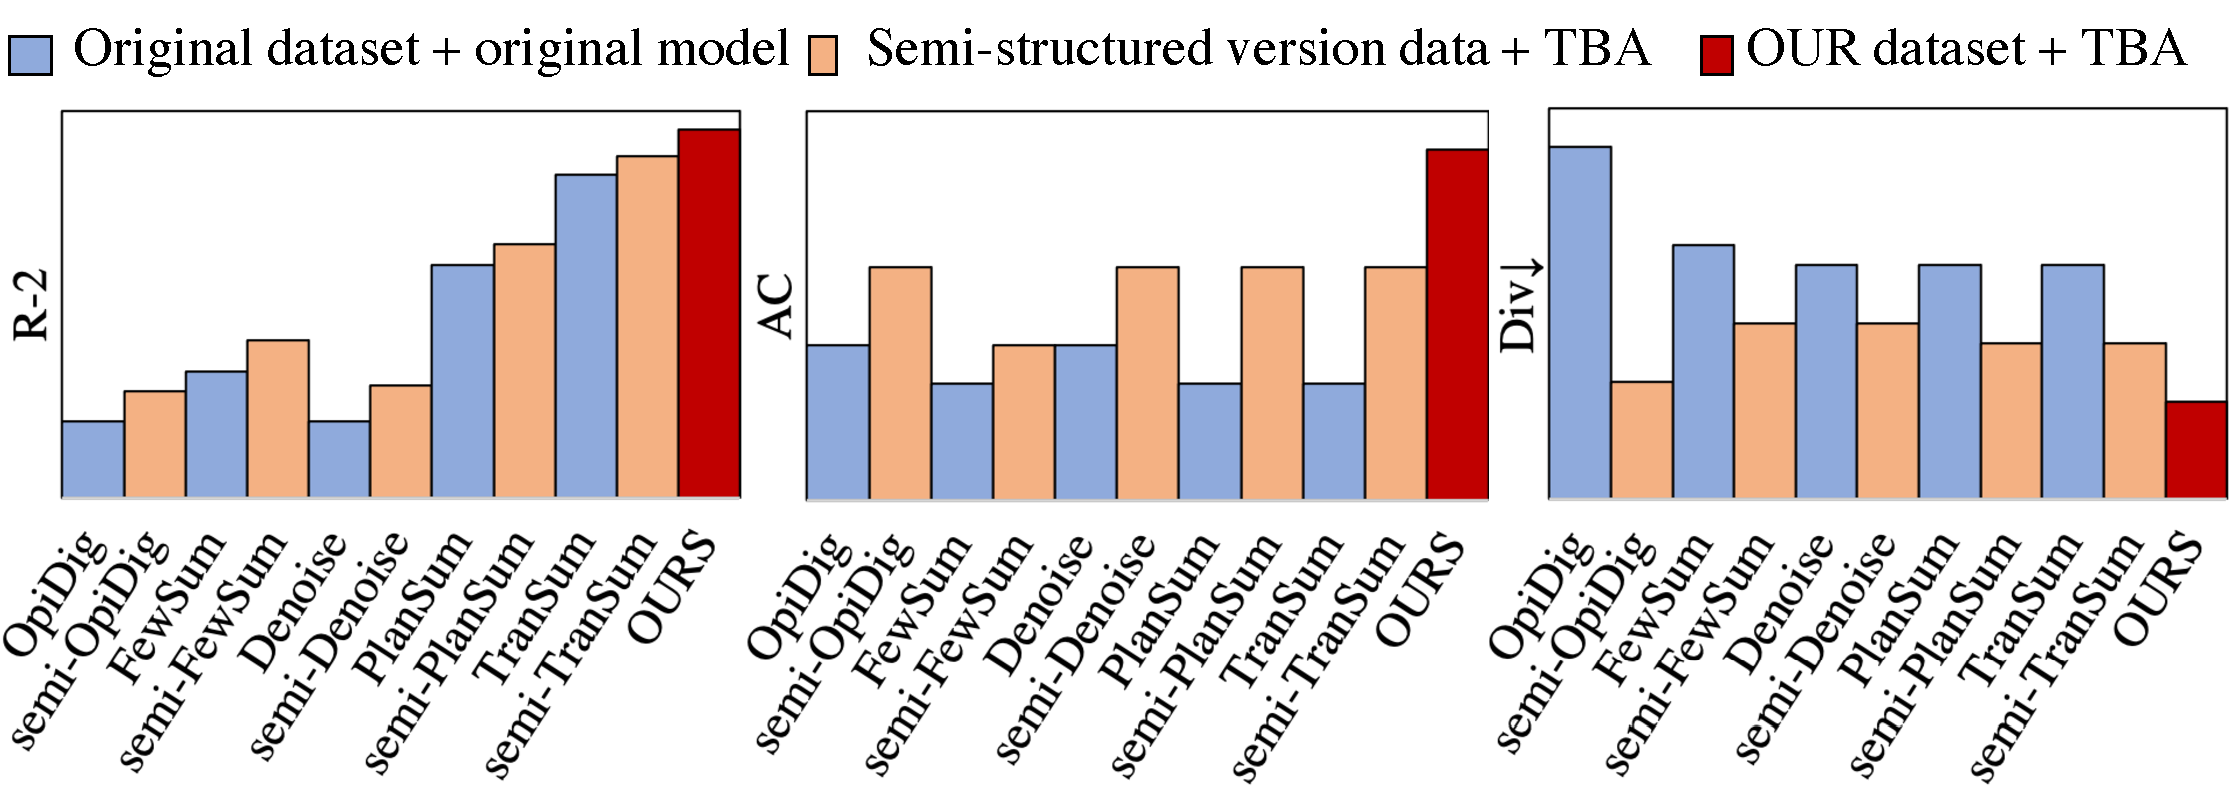
\includegraphics[width=1\linewidth]{ABL_data_Yelp.pdf}
		%\end{minipage}
	}
\subfigure[R-2, AC and Div$\downarrow$ scores of generated summaries in Amazon]{
	\label{fig:da}
	%\begin{minipage}[t]{0.33textwidth}
	\centering
	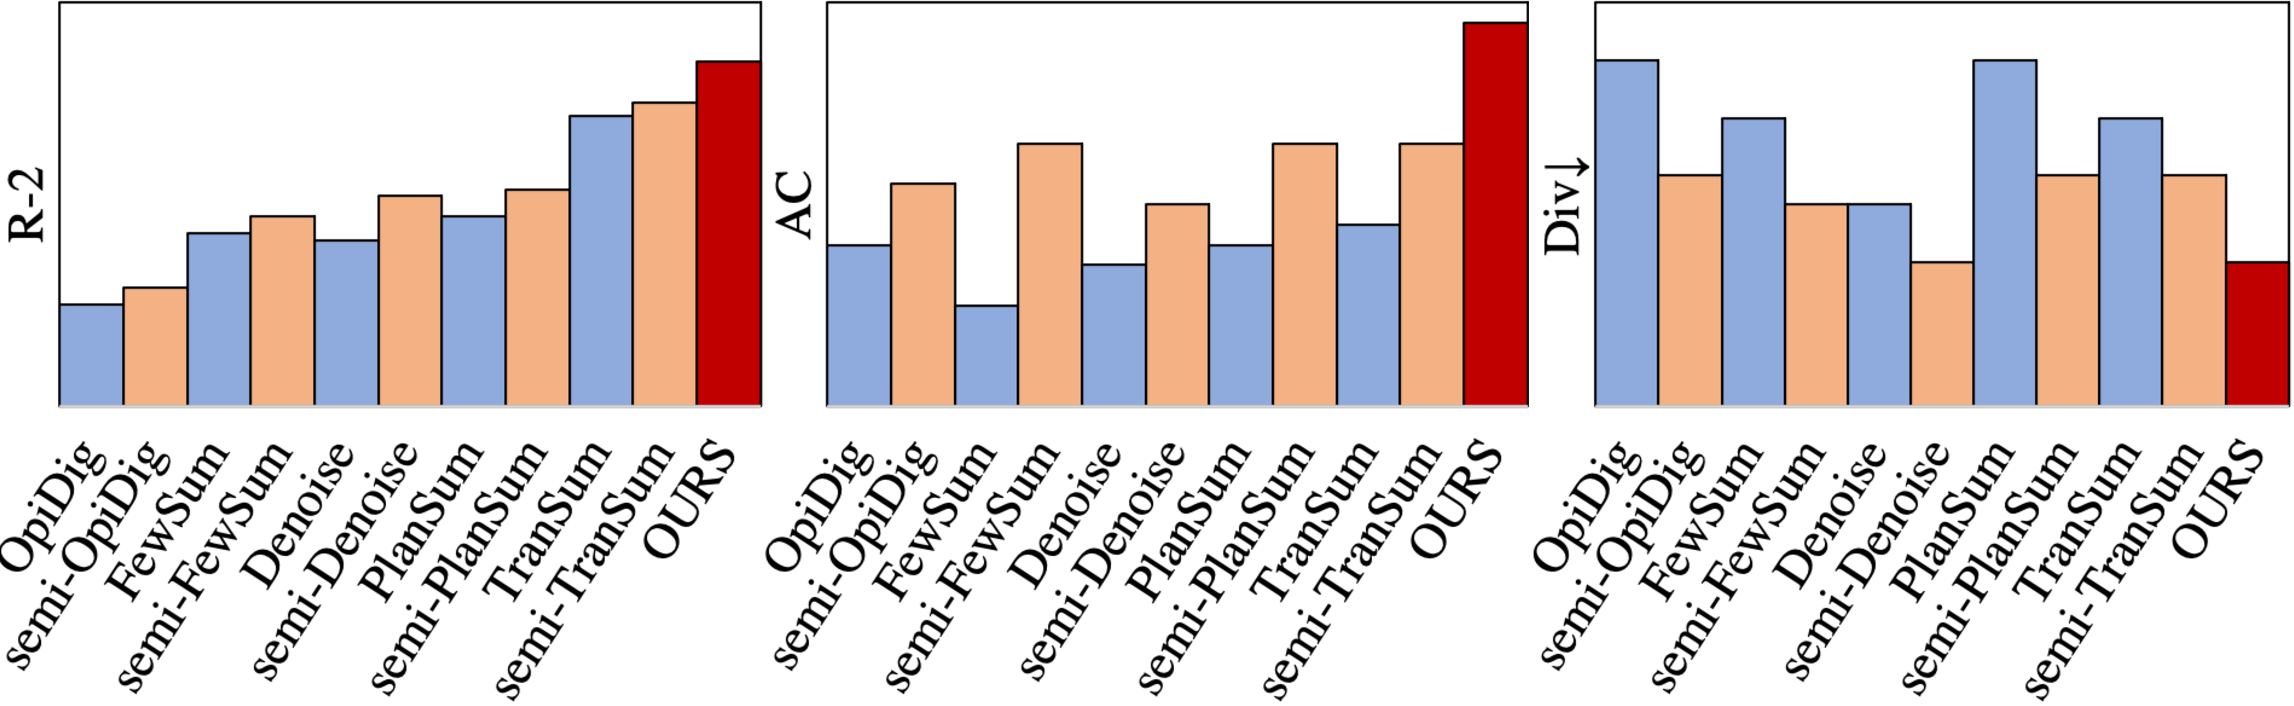
\includegraphics[width=1\linewidth]{ABL_data_Amazon.pdf}
	%\end{minipage}
}
\subfigure[R-2, AC and Div$\downarrow$ scores of generated summaries in RT]{
	\label{fig:dr}
	%\begin{minipage}[t]{0.33textwidth}
	\centering
	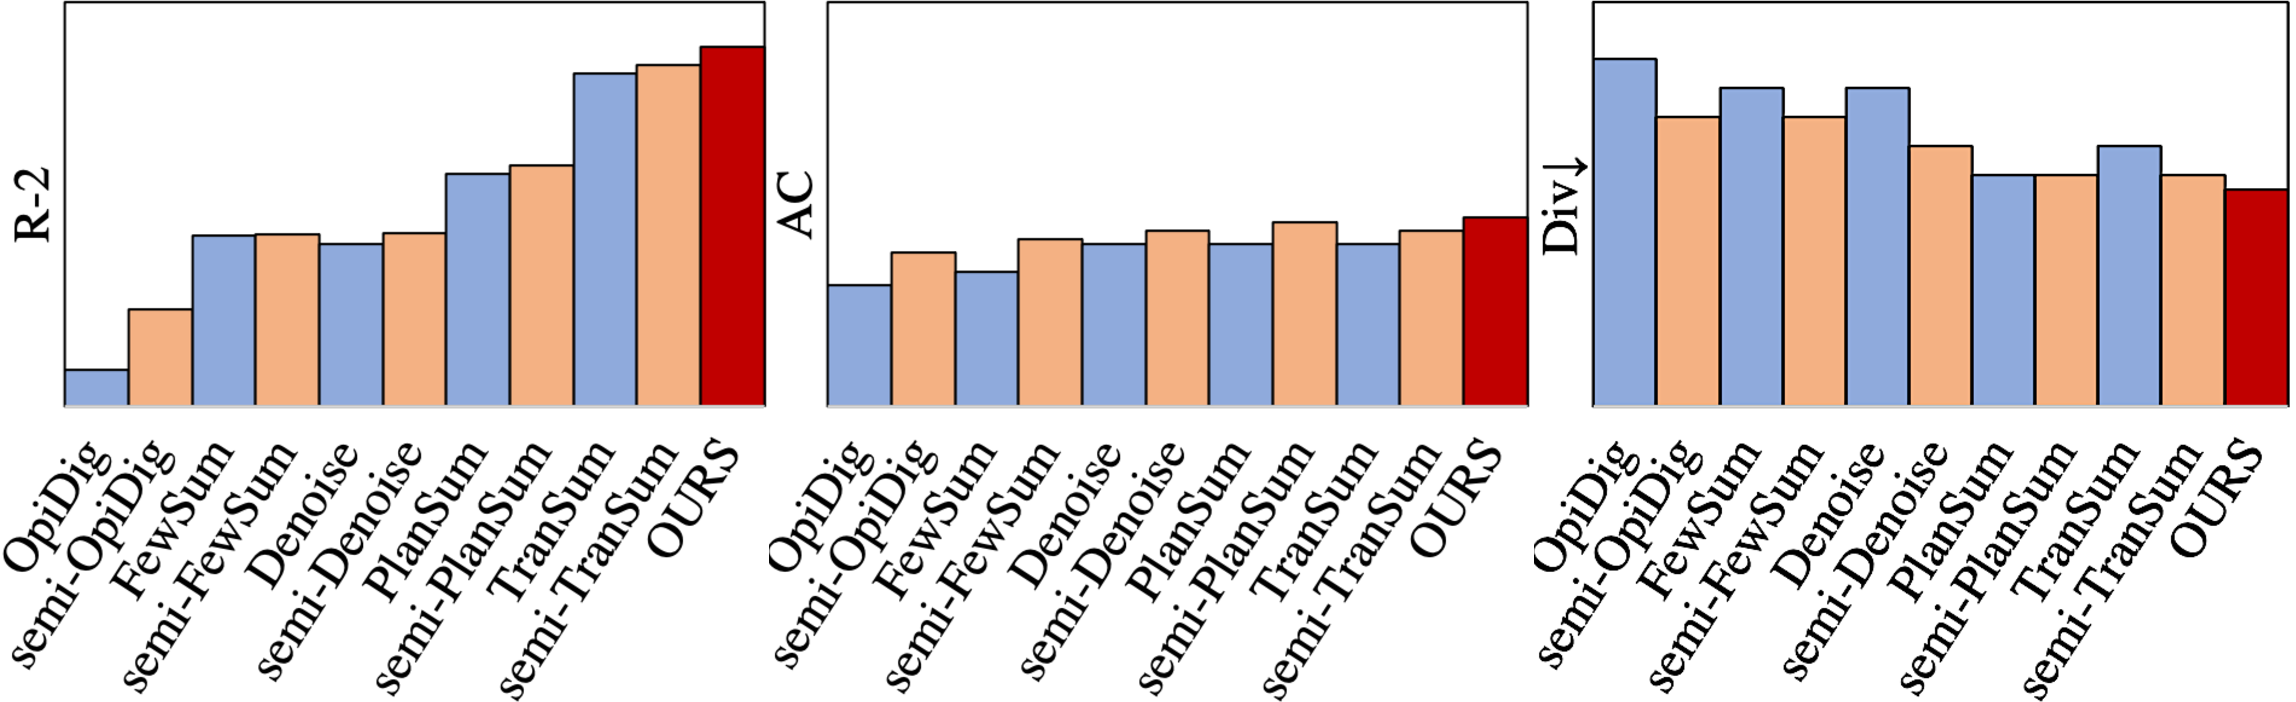
\includegraphics[width=1\linewidth]{ABL_data_RT.pdf}
	%\end{minipage}
}
	\caption{Results on three datasets using different synthetic data and their applicable models. The synthetic datasets in semi-structured version
		use TBA for training because of the characteristics of semi-structured data. ``semi-'' means semi-structured version. The data of TransSum is from {\em leave-one-out}. OURs denotes TBA-B trained on our created semi-structured synthetic data.}
	\label{fig:abl_data}
\end{figure}

According to different original synthetic datasets, we adopt different models for training.
This is because a synthetic dataset must be accompanied by its compatible model.
For the datasets with textual multi-review as input (FewSum, Denoise, PlanSum and TransSum), 
we convert them into semi-structured versions by extracting 
opinion-aspect pairs (OAs) and implicit sentences (ISs)
from their multi-reviews as input.
For the synthetic data with structured input (OpiDig),
we construct its semi-structured version
by generating the noisy OAs and noisy ISs for each output in original dataset and taking generated noisy OAs and ISs as input.
To be fair, for OpiDig, FewSum and Denoise,
the training on their original textual datasets did not use any pretrained language model,
so we train TBA-T without pretrained language models on their datasets in semi-structured version.
For semi-structured version data of PlanSum and TranSum,
we train TBA-B with pretrained language model on them,
as PlanSam and TranSum trained on original textual data used pretrained language model to import external knowledge.
In \figref{fig:abl_data},
TBA trained on the semi-structured version of previous textual synthetic datasets
is better than previous approaches in terms of R-2, AC and Div$\downarrow$ scores on all datasets,
showing that semi-structured data
is helpful in highlighting the aspects and opinions.
Compared with the structured datasets OpiDig, the semi-OpiDig get better ROUGE scores and Div$\downarrow$ scores as the ISs in semi-structured data help the model capture implicit information.


A review contains two types of sentences: the sentences  that can extract OAs (OA-sents) and the sentences that cannot extract OAs  (ISs) .
In our approach, we convert reviews into semi-structured version
to create synthetic training data.
To demonstrate that OAs don't lose the information of OA-sents,
we remove OAs and stopwords from OA-sents and compute the percentage of the rest tokens in original OA-sents. 
Experiments show that OA-sents have few words left 
with OAs and stop-words removed. 
Specifically, Yelp is $10.7\%$, Amazon is $11.1\%$, and RT is $4.3\%$. 
We also randomly sample 100 reviews from each dataset and ask human annotators to count the sentences that still contain useful information after removing OAs.
Human evaluation shows that $<10\%$ of OA-sents contain useful residual information, i.e., $9.1\%$ (Yelp), $9.3\%$ (Amazon), $4.0\%$ (RT).
The above results show that OA-sents contain very little implicit information.
Therefore, we take extract OAs from reviews as part of the input is reasonable.
As shown in \tabref{tab:OAIS}, 
we calculate the distribution of OA-sents and ISs in multi-reviews and reference summaries in human-annotated test sets.
Only using OAs as input will miss out the much information of multi-review
as the proportion of ISs in multi-review is more than $40\%$.
More than $30\%$ of sentences in reference summary are ISs, which should be summarized from the ISs in multi-review.
Thus, adding ISs is important and necessary.
\begin{table}[th]
	\small
	\centering
	\begin{tabular}{|l|cc|cc|}
		\hline
		\multirow{2}{*}{Dataset}&\multicolumn{2}{c|}{\textbf{Multi-review}}&\multicolumn{2}{c|}{\textbf{Reference summary}} \\ \cline{2-5}
		&OA-sents & ISs & OA-sents & ISs \\
		\hline
		Yelp & 0.54& 0.46&0.68 &0.32\\
		%\hline
		Amazon &  0.55&0.45&0.63&0.37\\
		%\hline
		RT &  0.33&0.67&0.32&0.68\\
		\hline
	\end{tabular}
	\caption{The proportion of OA-sent and IS in the test sets.}
	\label{tab:OAIS}
\end{table}

%\KZ{this para is a bit verbose. Cut!}
To investigate the importance of the individual components of semi-structured data, we perform ablations 
by only taking noisy OAs as input and only taking noisy IS as input.
We train BM on synthetic data with only noisy OAs or ISs as input,
and train TBA on data with both noisy OAs and ISs as input. 
Because we should deal with OAs and ISs in different ways. 
\tabref{tab:abl_comp} shows the results of taking both noisy OAs and ISs as input are the best on all evaluation metrics. 
Without noisy ISs as input, 
our approaches obtain worse R-2 and Div$\downarrow$ scores,
because the various implicit information of ISs is useful for R-2 and Div$\downarrow$.
Without noisy OAs as input, our approach gets worse in R-2 and AC  since OAs with explicit opinions and aspects are very important for opinion summarization.
We also compare matched (MA) OAs and mismatched (MM) OAs in noisy OAs.
%we train our models on the datasets only taking MA OAs as input and MM OAs as input.
%As noisy OAs contain matched (MA) OAs and mismatched (MM) OAs, %we also compare the performance of training with only EM OAs as input and MM OAs as input.
The models with only MM OAs as input have bad performance
due to introducing much redundant information.
Taking both MA and MM OAs as input performs better than taking only MA OAs as input
since the noisy OAs containing MA and MM OAs is more similar to the OAs distribution in actual multi-review.
The complete noisy OAs help model learning capture important aspects and opinions.% from multi-reviews.
For RT dataset, as shown in \figref{fig:dr}, 
the difference between the results of the original methods and their semi-structured version is less than that of other datasets. 
As shown in \tabref{tab:abl_comp}, different from Yelp and Amazon,
RT is more impacted by noisy ISs than noisy OAs.
Movie reviews in RT contain discussion on plot, such as the Gold in \tabref{tab:overall_exp}(b),
and the proportion of OA-sent in RT becomes less (in  \tabref{tab:OAIS}), 
which makes the handling of OAs in our approaches not fully utilized.
\begin{table}[th]
	\centering
	\small
	\begin{tabular}{|p{0.25cm}p{0.25cm}p{0.25cm}p{0.55cm}m{1.55cm}<{\centering}m{1.55cm}<{\centering}m{1.55cm}<{\centering}|}
		\hline
		MA & MM & IS & \bf Model & \bf Yelp & \bf Amazon & \bf RT \\
		\hline
		$\checkmark$ & $\checkmark$ & $\checkmark$ &TBA& \bf 8.76/0.44/0.20 & \bf 7.84/0.34/0.25 & \bf 9.07/0.17/0.23 \\
		$\checkmark$ &  & $\checkmark$&TBA& 7.43/0.42/0.20 & 6.92/0.30/0.26 & 7.90/0.17/0.24 \\
		& $\checkmark$ & $\checkmark$&TBA & 3.73/0.23/0.22 & 3.48/0.22/0.25& 6.44/0.14/0.24  \\
		\hline
		$\checkmark$ & $\checkmark$ & & BM& 6.83/0.40/0.25& 6.31/0.28/0.27 & 2.71/0.16/0.25  \\
		$\checkmark$ &  & & BM & 5.38/0.36/0.28& 5.33/0.26/0.28 & 2.43/0.15/0.27 \\
		& $\checkmark$ & & BM & 3.24/0.13/0.30 & 2.98/0.15/0.28& 1.29/0.10/0.33 \\
		\hline
		& & $\checkmark$ & BM & 3.95/0.24/0.24 & 3.66/0.24/0.23& 6.45/0.14/0.24  \\
		\hline
	\end{tabular}
	\caption{Ablation study on individual components of semi-structured input. 
		Noisy OAs contains matched (MA) OAs and mismatched (MM) OAs. IS is noisy ISs. 
		Each row shows the R-2/AC/Div$\downarrow$ scores of the  BART-based model trained on the components annotated by ``$\checkmark$''.}
	\label{tab:abl_comp}
\end{table}

In general, TBA trained on semi-structured synthetic dataset (OURS) achieves the best scores in \figref{fig:abl_data} and \tabref{tab:abl_comp}. This shows that the way of getting noisy OAs and ISs according to sampled summary is optimal.
Our proposed semi-structured approach is more effective on the reviews with explicit opinion information (OAs), such as the reviews of products, places or services.

\textbf{Our proposed models.}
As shown in \tabref{tab:abla},
we compare different models designed for semi-structured training data.

BM with noisy OAs as input performs worst,
as BM only learns to make sentences from OAs. 
At test, BM can only generate summaries
from the OAs in multi-review and cannot capture the information of sentence without OAs. 
\tabref{tab:overall_exp} shows that the sentences in BM summary
are in general and have no specific information.

AM deals with OAs and ISs by different encoders, which performs better than BM on all evaluation metrics. 
As shown in \tabref{tab:overall_exp}, 
AM makes sentences from OAs better and generates more sentences summaried from ISs.
The AC scores models in \tabref{tab:abla} are similar between BM and AM of Yelp and Amazon
because the reviews in these two datasets contain much more OAs
and these two models directly use the same noisy OAs as input.
However, for RT, AM models are greatly improved after introducing noisy ISs, because the movie reviews contain less OAs and more ISs, 
as shown in \tabref{tab:overall_exp}(c) and \tabref{tab:OAIS}.

To make full use of semi-structured data,
TBA is the model first trained on BM and then fine-tuned on AM.
The pretraining of TBA on AM enables the model better to select OAs. 
The OAs of TBA in \tabref{tab:overall_exp} are most similar to Gold.
The last sentence of TBA output in \tabref{tab:overall_exp}(a) is inferred by adding ISs.
TBA obtains the best results on all datasets, which shows
that the way of training the semi-structured data on 
the model with a dual encoder is effective. 
Compared with gold summary, the sentence in generated summaries are not coherent enough 
and the coreference is not clear. For example, in \tabref{tab:overall_exp}(a), the sentences in TBA output 
on food are incoherent and the `it' in the last sentence denotes the restaurant. The reason is that some reviews in corpus are abbreviated or nonstandard, which brings the noise to the datasets and models.

We observe the performance of the models on different datasets.
BM performs badly on RT since BM focuses on OAs while OAs are less in BM.
After using ISs, AM trained on RT improves most because the movie reviews in RT contains more ISs, such as character and plot descriptions.
TBA performs better than AM because of the pretraining on BM.
The difference between TBA and AM trained on Yelp and Amazon is greater than that trained on RT, 
because Yelp and Amazon contain more OAs than RT.
The pretrained BM is more effective in Yelp and Amazon.
In summary, our proposed approaches are more sensitive to 
explicit opinion information. 
%\KZ{Rather u should point out that BM does very badly on RT, and why?}


\begin{table}[th]
	\centering
	\small
		\begin{tabular}{|l|l|ccc|}
			\hline
			\multicolumn{2}{|c|}{\bf Model} & \bf Yelp & \bf Amazon & \bf RT \\ 
			\hline
			\multirow{3}{*}{Trans} & BM & 5.37/0.35/0.26& 5.42/0.26/0.38& 2.18/0.15/0.27 \\
			& AM & 5.55/0.33/0.24 & 5.73/0.24/0.27& 4.92/0.14/0.25\\
			& TBA & \bf 6.07/0.41/0.22 & \bf 6.19/0.33/0.26 & \bf 5.23/0.17/0.24 \\
			\hline
			\multirow{3}{*}{BART} & BM & 6.83/0.40/0.25 & 6.31/0.28/0.27 & 2.71/0.16/0.25 \\
			& AM & 7.94/0.38/0.22 & 7.23/0.28/0.26 & 8.93/0.16/0.23\\
			& TBA & \bf 8.76/0.44/0.20 & \bf 7.84/0.34/0.25 & \bf 9.07/0.17/0.23 \\
			\hline
		\end{tabular}
	\caption{R-2/AC/Div$\downarrow$ of summaries generated by transformer (Trans) and BART training on our synthetic data.}	\label{tab:abla}
\end{table}

\cut{%%%%%%
\begin{table}[th]
	\centering
	\small
	\subtable[Aspect Coverage and Diversity scores]{
		%\label{tab:abla}  
	
	\begin{tabular}{|l|l|c|c|c|c|}
	\hline
	\multicolumn{2}{|c|}{\multirow{2}{*}{\bf Model}} & \multicolumn{2}{c|}{\bf Yelp} &  \multicolumn{2}{c|}{\bf Amazon} \\ \cline{3-6}
	\multicolumn{2}{|c|}{} & AC & Div & AC & Div \\
	\hline
	\multirow{4}{*}{Trans} & BAG & 0.35 & 0.26  & 0.26& 0.28 \\
	& BAI & 0.33 & 0.24 &0.24 & 0.27 \\
	%& MAI & 0.39&  0.23 & 0.30 & 0.26 \\
	& MB & \bf 0.41 & \bf 0.22 & \bf 0.33 & \bf 0.26\\
	\hline
	\multirow{4}{*}{BART} & BAG &0.40 & 0.25 &0.28 & 0.27 \\
	& BAI & 0.38 & 0.22 & 0.28 & 0.26 \\
	%& MAI & 0.43 & 0.22 & 0.32 & 0.26 \\
	& MB & \bf 0.44 & \bf 0.20 &\bf 0.34 & \bf 0.25 \\
	\hline
\end{tabular}
	}
\qquad
\subtable[ROUGE scores]{
	%\label{tab:acdv}
\begin{tabular}{|l|m{0.7cm}<{\raggedright}|m{0.6cm}<{\centering}|c|c|c|c|m{0.6cm}<{\centering}|}
	\hline
	\multicolumn{2}{|c|}{\multirow{2}{*}{\bf Model}} & \multicolumn{3}{c|}{\bf Yelp} &  \multicolumn{3}{c|}{\bf Amazon} \\ \cline{3-8}
	\multicolumn{2}{|c|}{}& R-1 & R-2 & R-L & R-1 & R-2 & R-L\\
	\hline
	\multirow{4}{*}{Trans}&BAG & 30.78 & 5.37 & 17.38 & 29.20 & 5.42 & 17.96 \\
	&BAI & 32.09 & 5.55 & 17.60 & 30.27 & 5.73& 18.39 \\
	%&MAI & 32.21 & 5.71 & 18.06 & 31.94 & 6.00& 19.69\\
	&MB & \bf 33.43 & \bf 6.07  & \bf 18.37 & \bf 32.57 &\bf 6.19 & \bf 20.18 \\
	\hline
	\multirow{4}{*}{BART}&BAG & 34.79 & 6.83 & 18.42 & 31.27 & 6.31 & 19.14  \\
	&BAI & 36.27 & 7.94  & 20.60 & 33.96 & 7.23 &20.77 \\
	%&MAI & 36.93 & 8.40  & 21.11 & 34.47& 7.57& 21.03\\
	&MB & \bf 37.58 & \bf 8.76 & \bf 21.17 & \bf 35.30 & \bf 7.84 & \bf 21.33  \\
	\hline
\end{tabular}
}
\caption{The results of summaries generated by transformer (Trans) and BART training on our synthetic training data.}	\label{tab:abla}
\end{table}
}%%%%%%%%





